%% 美赛模板:正文部分

\documentclass[12pt]{article}  % 官方要求字号不小于 12 号,此处选择 12 号字体
% 本模板不需要填写年份,以当前电脑时间自动生成
% 请在以下的方括号中填写队伍控制号
\usepackage[000000]{easymcm}  % 载入 EasyMCM 模板文件
\problem{CEF}  % 请在此处填写题号
 \usepackage{mathptmx}  % 这是 Times 字体,中规中矩 
%\usepackage{mathpazo}  % 这是 COMAP 官方杂志采用的更好看的 Palatino 字体,可替代以上的 mathptmx 宏包
\title{{\sc Our Title}\\ Our Title}  % 标题
\usepackage{enumerate}
\usepackage{lettrine}
\usepackage[ruled,linesnumbered]{algorithm2e}
\usepackage{lipsum}
\usepackage{hyperref}
\usepackage{adjustbox}
% 如需要修改题头(默认为 MCM/ICM),请使用以下命令(此处修改为 MCM)
%\renewcommand{\contest}{MCM}
\usepackage{bm}
\usepackage{cleveref}
\usepackage{ulem}
\usepackage{geometry}
\usepackage{framed} 
\usepackage{mathrsfs}
\usepackage{lettrine}
\usepackage{wasysym}
% 文档开始
\begin{document}

% 此处填写摘要内容
\begin{abstract}

    \vspace{5pt}
    \textbf{Keywords}:

\end{abstract}

\maketitle  % 生成 Summary Sheet
\tableofcontents  % 生成目录


% 正文开始
\section{Introduction}
\subsection{Background}

\subsection{Restatement of the Problem}
\begin{enumerate}[\textbf{problem} 1 ]
\item text
\end{enumerate}
\subsection{Our Work}
{\LARGE\CheckedBox} 

 Here's our work:
\begin{figure}[htbp]
\centering
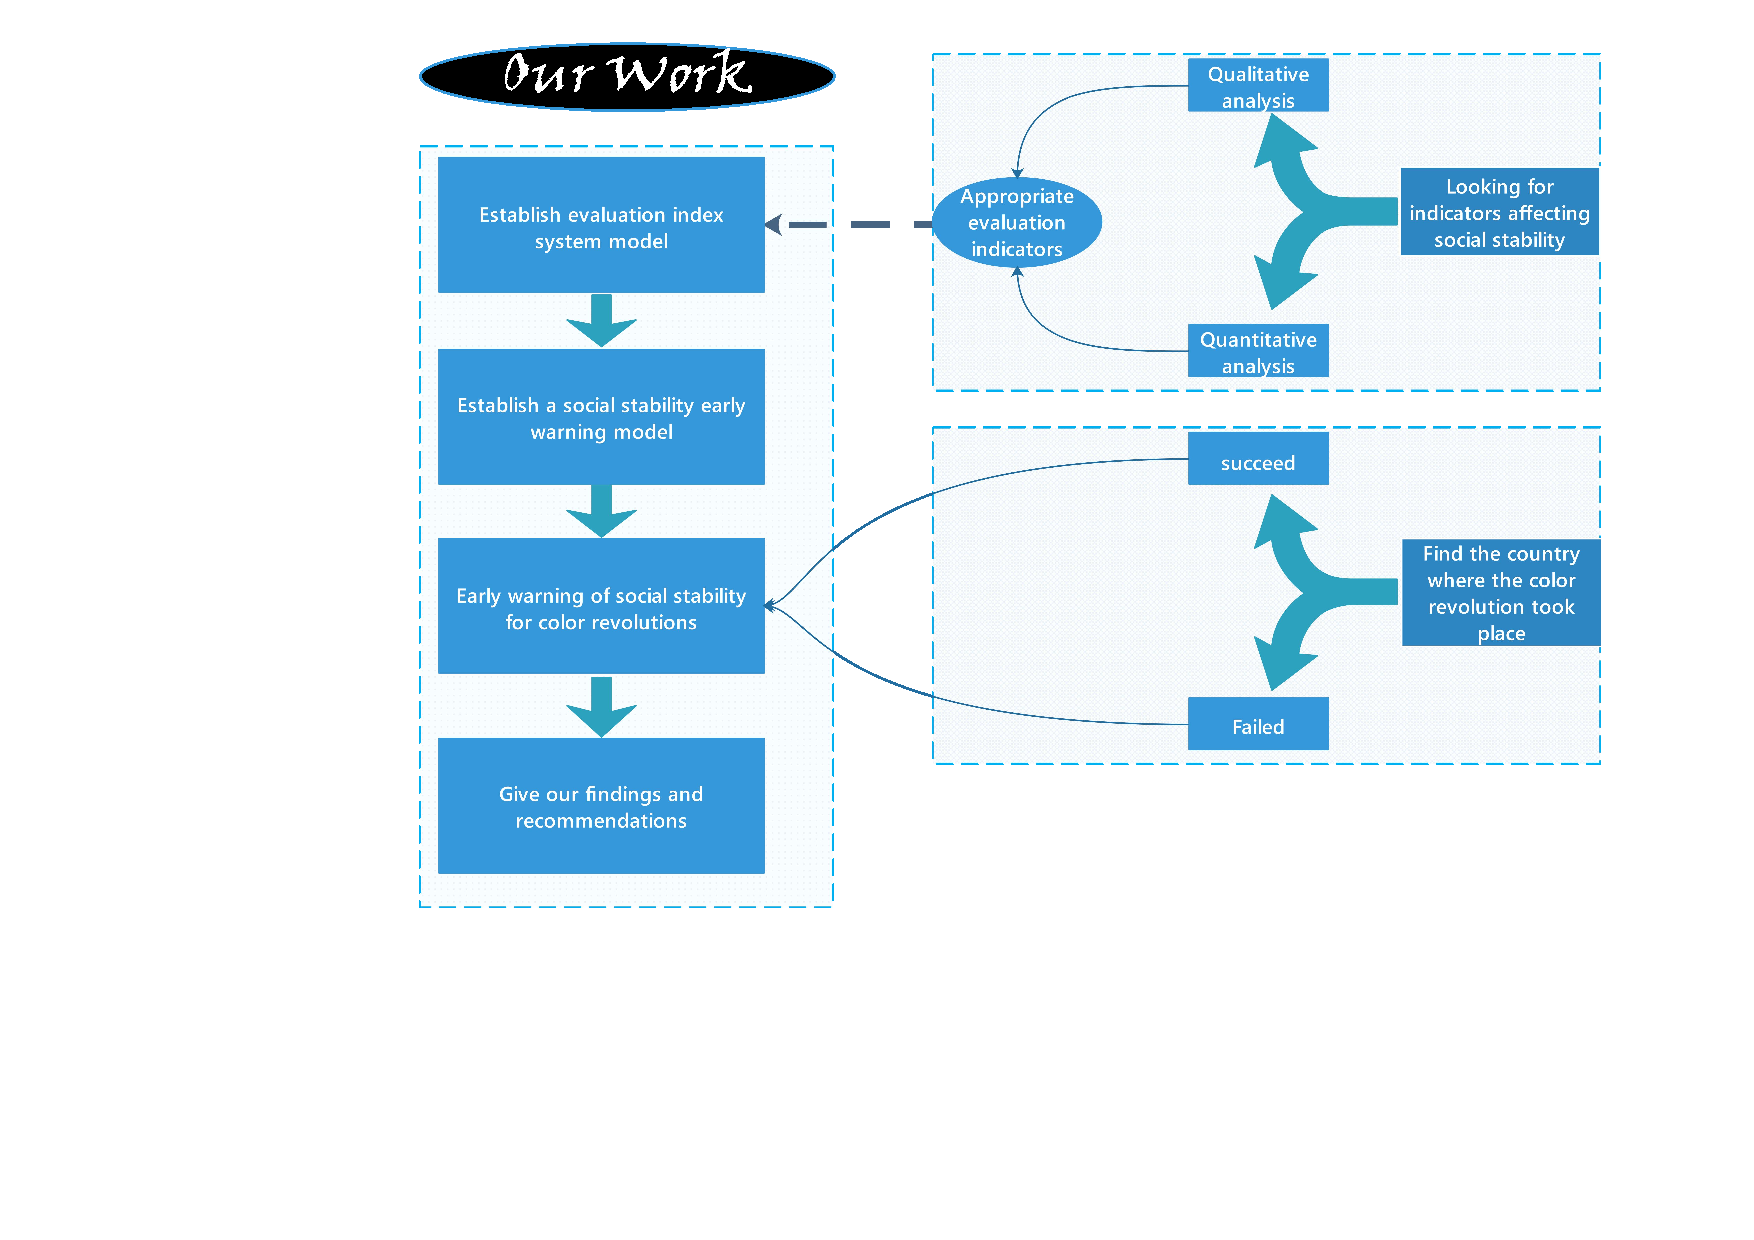
\includegraphics[width=.4\textwidth]{img/our work.pdf}
\caption{Our Work}
\end{figure}


\section{Assumptions and Notations}
\subsection{Assumptions}
To simplify our model, this paper makes following basic assumption, each of which is properly
justified.
\begin{itemize}
	\item We assume that

	$\hookrightarrow$ \textbf{Justification:} Justification
\end{itemize}
\subsection{Notations}
Notations that we use in the model are shown in the Table \ref{tb:notation}:
% 三线表示例
\begin{table}[!htbp]
\begin{center}
\caption{Notations}
\begin{tabular}{clc}
	\toprule[1.5pt]
	% \multicolumn{1}{m{3cm}}
	{\centering {\itshape\textbf{Symbol}}}
	&
	% \multicolumn{1}{m{8cm}}
	{\itshape\textbf{Description}}&{\centering {\itshape\textbf{Unit}}} \\
	\midrule
	$A_i$&Level 1 indicators&- \\
	\bottomrule[1.5pt]
\end{tabular}\label{tb:notation}
\end{center}
\end{table}












\section{Establishment of Our Model}
\subsection{Model I}

\begin{enumerate}
    \renewcommand{\labelenumi}{\textbf{Step \theenumi}}
    \item 

\end{enumerate}



































































\section{Solution For Problem One}
% \subsection{subsection}
% \begin{figure}[htbp]
% \centering
% \begin{subfigure}[b]{.32\textwidth}
% 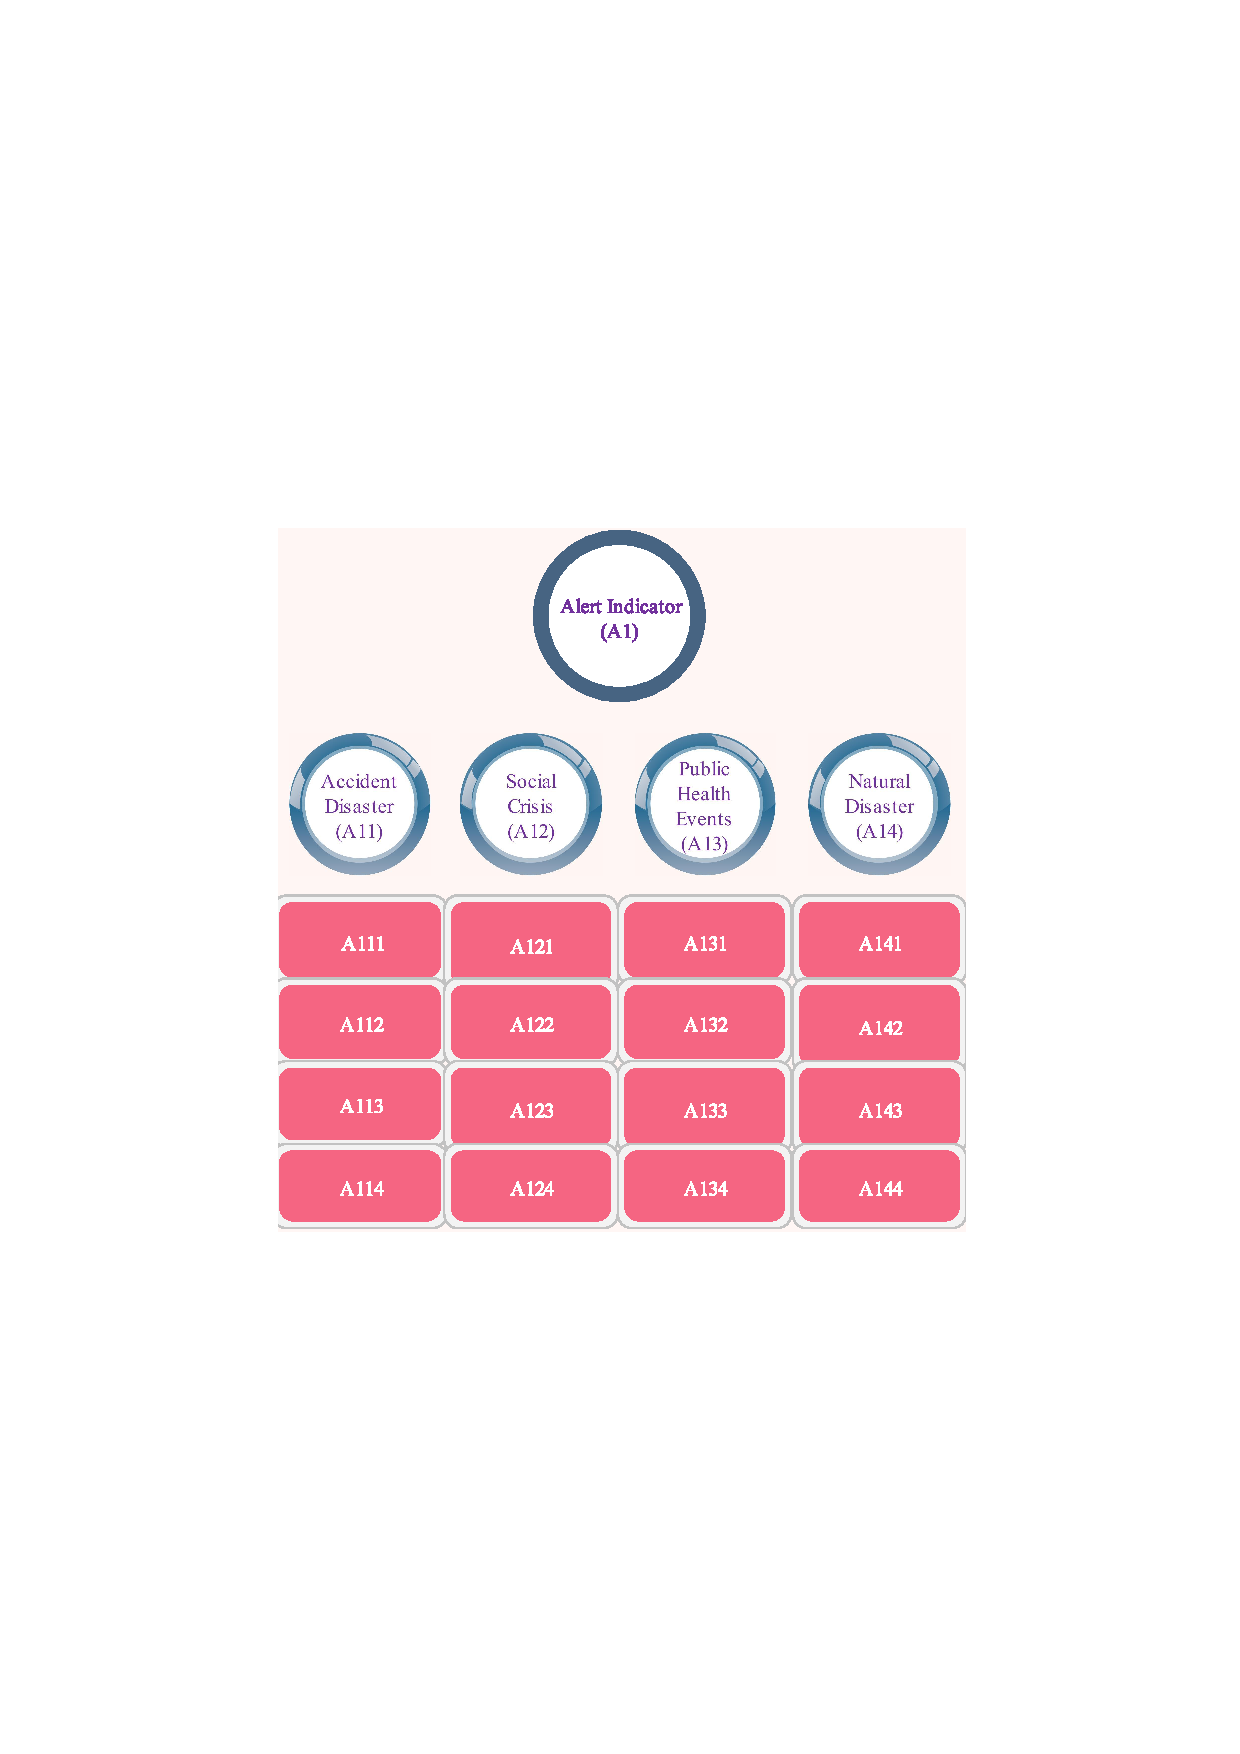
\includegraphics[width=\textwidth]{img/1.pdf}
% \end{subfigure}
% \begin{subfigure}[b]{.32\textwidth}
% 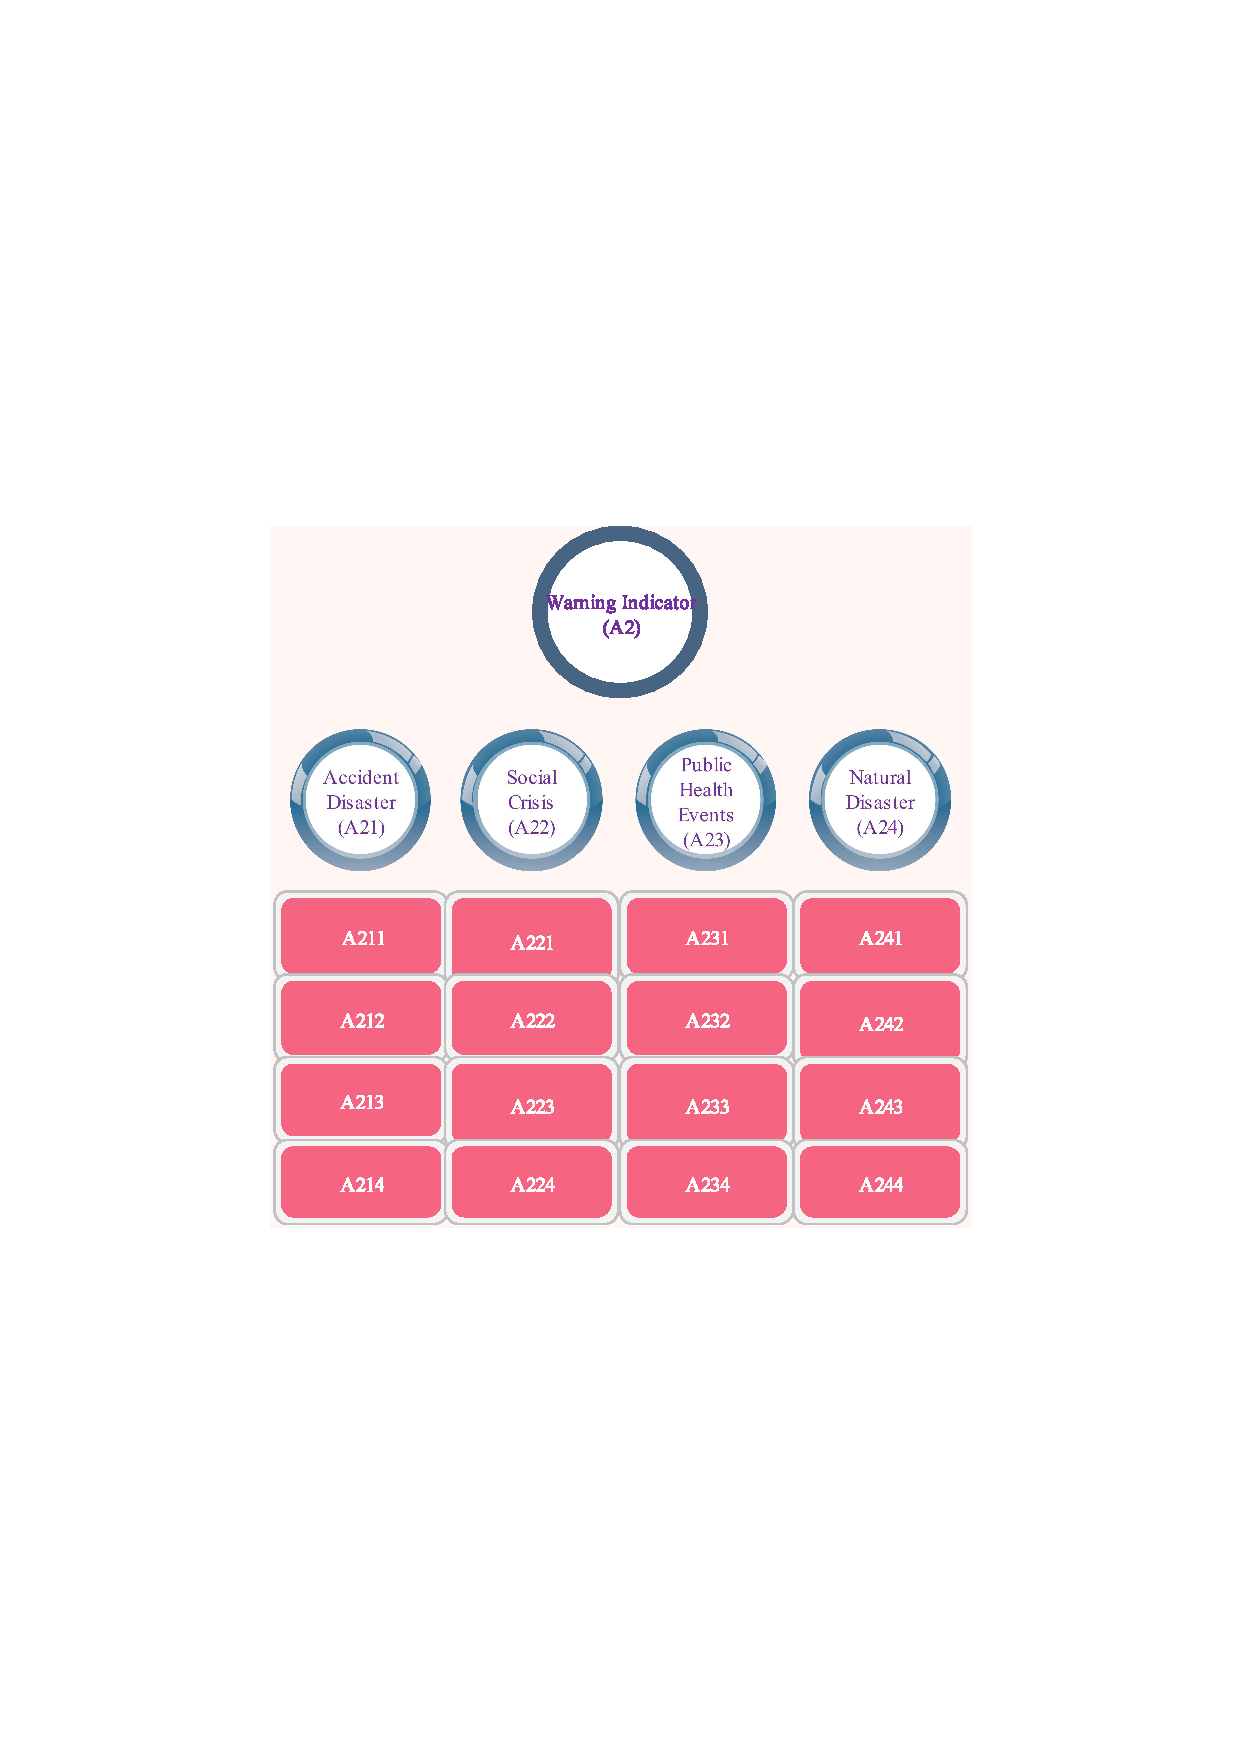
\includegraphics[width=\textwidth]{img/2.pdf}
% \end{subfigure}
% \begin{subfigure}[b]{.32\textwidth}
% 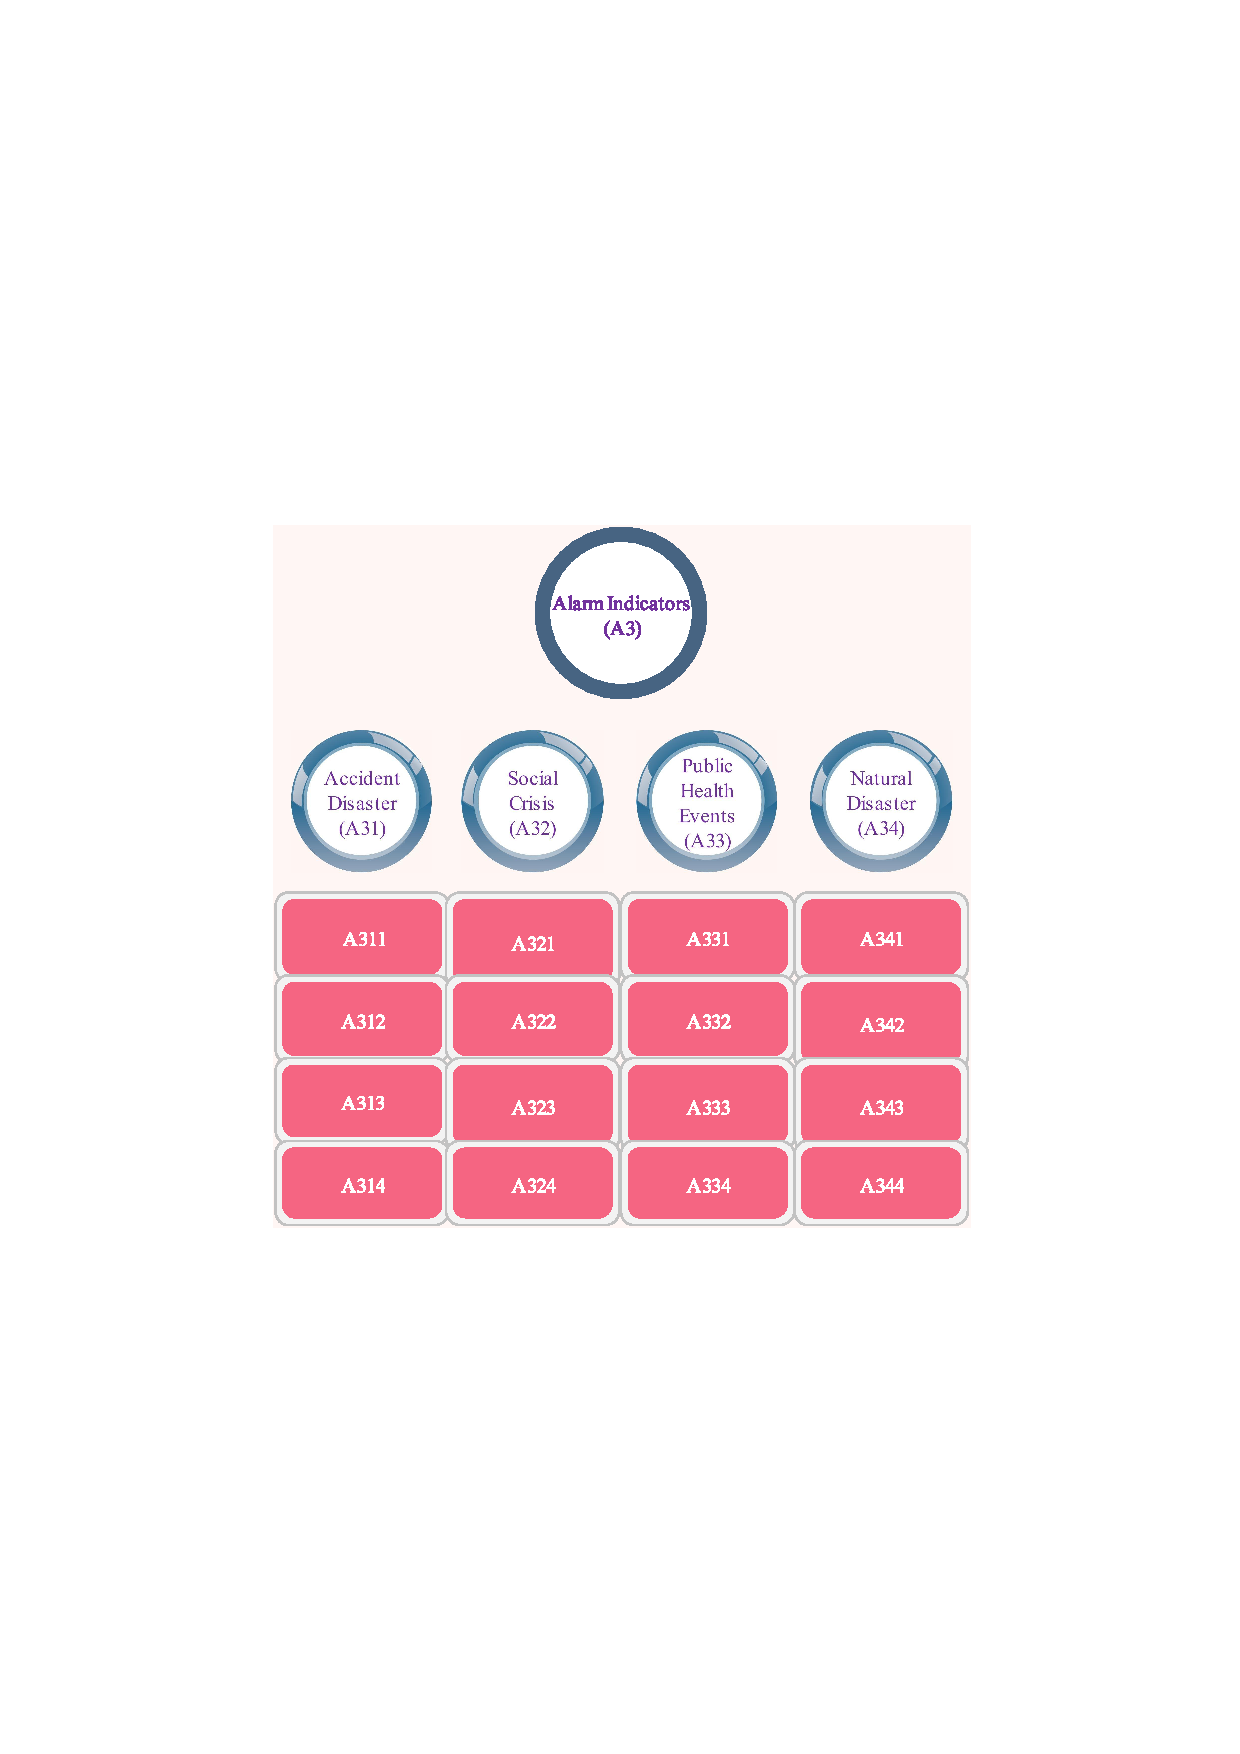
\includegraphics[width=\textwidth]{img/3.pdf}
% \end{subfigure}
% \caption{Your figure title}
% \end{figure}





\newpage
\section{Analysis and Promotion of Our Model}
\subsection{Sensitivity Analysis of Our Model}
\subsection{Strengths and Weaknesses}
Our research is basically based on the predecessors, and there are some improvements and shortcomings as follows:
\subsubsection{Strengths}
\subsubsection{Weaknesses}
\subsection{Future Work}























































% The instance of long and wide tables are shown in Table \ref{tb:longtable}.

% % 长表格示例,更多用法请参考 longtable 宏包文档
% % 以下环境及对应参数可实现表格内的自动换行与表格的自动断页
% % 您也可以选择自行载入 tabularx 宏包,并通过 X 参数指定对应列自动换行
% \begin{longtable}{ p{4em} p{14em} p{14em} }
% \caption{Basic Information about Three Main Continents (scratched from Wikipedia)}
% \label{tb:longtable}\\
% \toprule
% Continent & Description & Information \\
% \midrule
% Africa & Africa Continent is surrounded by the Mediterranean Sea to the
% north, the Isthmus of Suez and the Red Sea to the northeast, the Indian
% Ocean to the southeast and the Atlantic Ocean to the west. &
% At about 30.3 million km$^2$ including adjacent islands, it covers 6\%
% of Earth's total surface area and 20\% of its land area. With 1.3
% billion people as of 2018, it accounts for about 16\% of the world's
% human population. \\
% \midrule
% Asia & Asia is Earth's largest and most populous continent which
% located primarily in the Eastern and Northern Hemispheres.
% It shares the continental landmass of Eurasia with the continent
% of Europe and the continental landmass of Afro-Eurasia with both
% Europe and Africa. &
% Asia covers an area of 44,579,000 square kilometres, about 30\%
% of Earth's total land area and 8.7\% of the Earth's total surface
% area. Its 4.5 billion people (as of June 2019) constitute roughly
% 60\% of the world's population. \\
% \midrule
% Europe & Europe is a continent located entirely in the Northern
% Hemisphere and mostly in the Eastern Hemisphere. It comprises the
% westernmost part of Eurasia and is bordered by the Arctic Ocean to
% the north, the Atlantic Ocean to the west, the Mediterranean Sea to
% the south, and Asia to the east. &
% Europe covers about 10,180,000 km$^2$, or 2\% of the Earth's surface
% (6.8\% of land area), making it the second smallest
% continent. Europe had a total population of about 741 million (about
% 11\% of the world population) as of 2018. \\
% \bottomrule
% \end{longtable}
















% 以下为信件/备忘录部分,不需要可自行去掉
% 如有需要可将整个 letter 环境移动到文章开头或中间
% 请在第二个花括号内填写标题,如「信件」(Letter)或「备忘录」(Memorandum)
\begin{letter}{\huge{$\mathscr{MEMO}$}}
\begin{flushleft}  % 左对齐环境,无首行缩进
\textbf{To:} MCM/ICM organizing committee\\
\textbf{From:} Team 000000\\
\textbf{Date:}\today\\
\textbf{Subject:} 
\end{flushleft}
\lettrine{T}{he}
{\itshape \begin{enumerate}[0]
    \item[$\bullet$] Keep a firm grip on the local media to prevent public opinion from getting out of control. There is no substitute for the role of the media in regime change, and its entry into and occupation of a country's position of public opinion can help to bring down that country's regime. For the ruling party, therefore, to give ground. That means the beginning of the loss of power, public opinion out of control, not much time.
\end{enumerate}}
\end{letter}
\begin{algorithm}
\caption{Simulation-optimization heuristic}\label{algorithm}
\KwData{current period $t$, initial inventory $I_{t-1}$, initial capital $B_{t-1}$, demand samples}
\KwResult{Optimal order quantity $Q^{\ast}_{t}$}
$r\leftarrow t$\;
$\Delta B^{\ast}\leftarrow -\infty$\;
\While{$\Delta B\leq \Delta B^{\ast}$ and $r\leq T$}{$Q\leftarrow\arg\max_{Q\geq 0}\Delta B^{Q}_{t,r}(I_{t-1},B_{t-1})$\;
$\Delta B\leftarrow \Delta B^{Q}_{t,r}(I_{t-1},B_{t-1})/(r-t+1)$\;
\If{$\Delta B\geq \Delta B^{\ast}$}{$Q^{\ast}\leftarrow Q$\;
$\Delta B^{\ast}\leftarrow \Delta B$\;}
$r\leftarrow r+1$\;}
\end{algorithm}
%伪代码








% \begin{figure}[h!] 	
% \vspace{-0.8cm}   %调整图片与上文的垂直距离  
% \setlength{\abovecaptionskip}{0.cm} %调整标题上方的距离   
% \setlength{\abovecaptionskip}{0.cm} %调整标题下方的距离 	   
% \setlength{\belowdisplayskip}{0.pt} 	
% 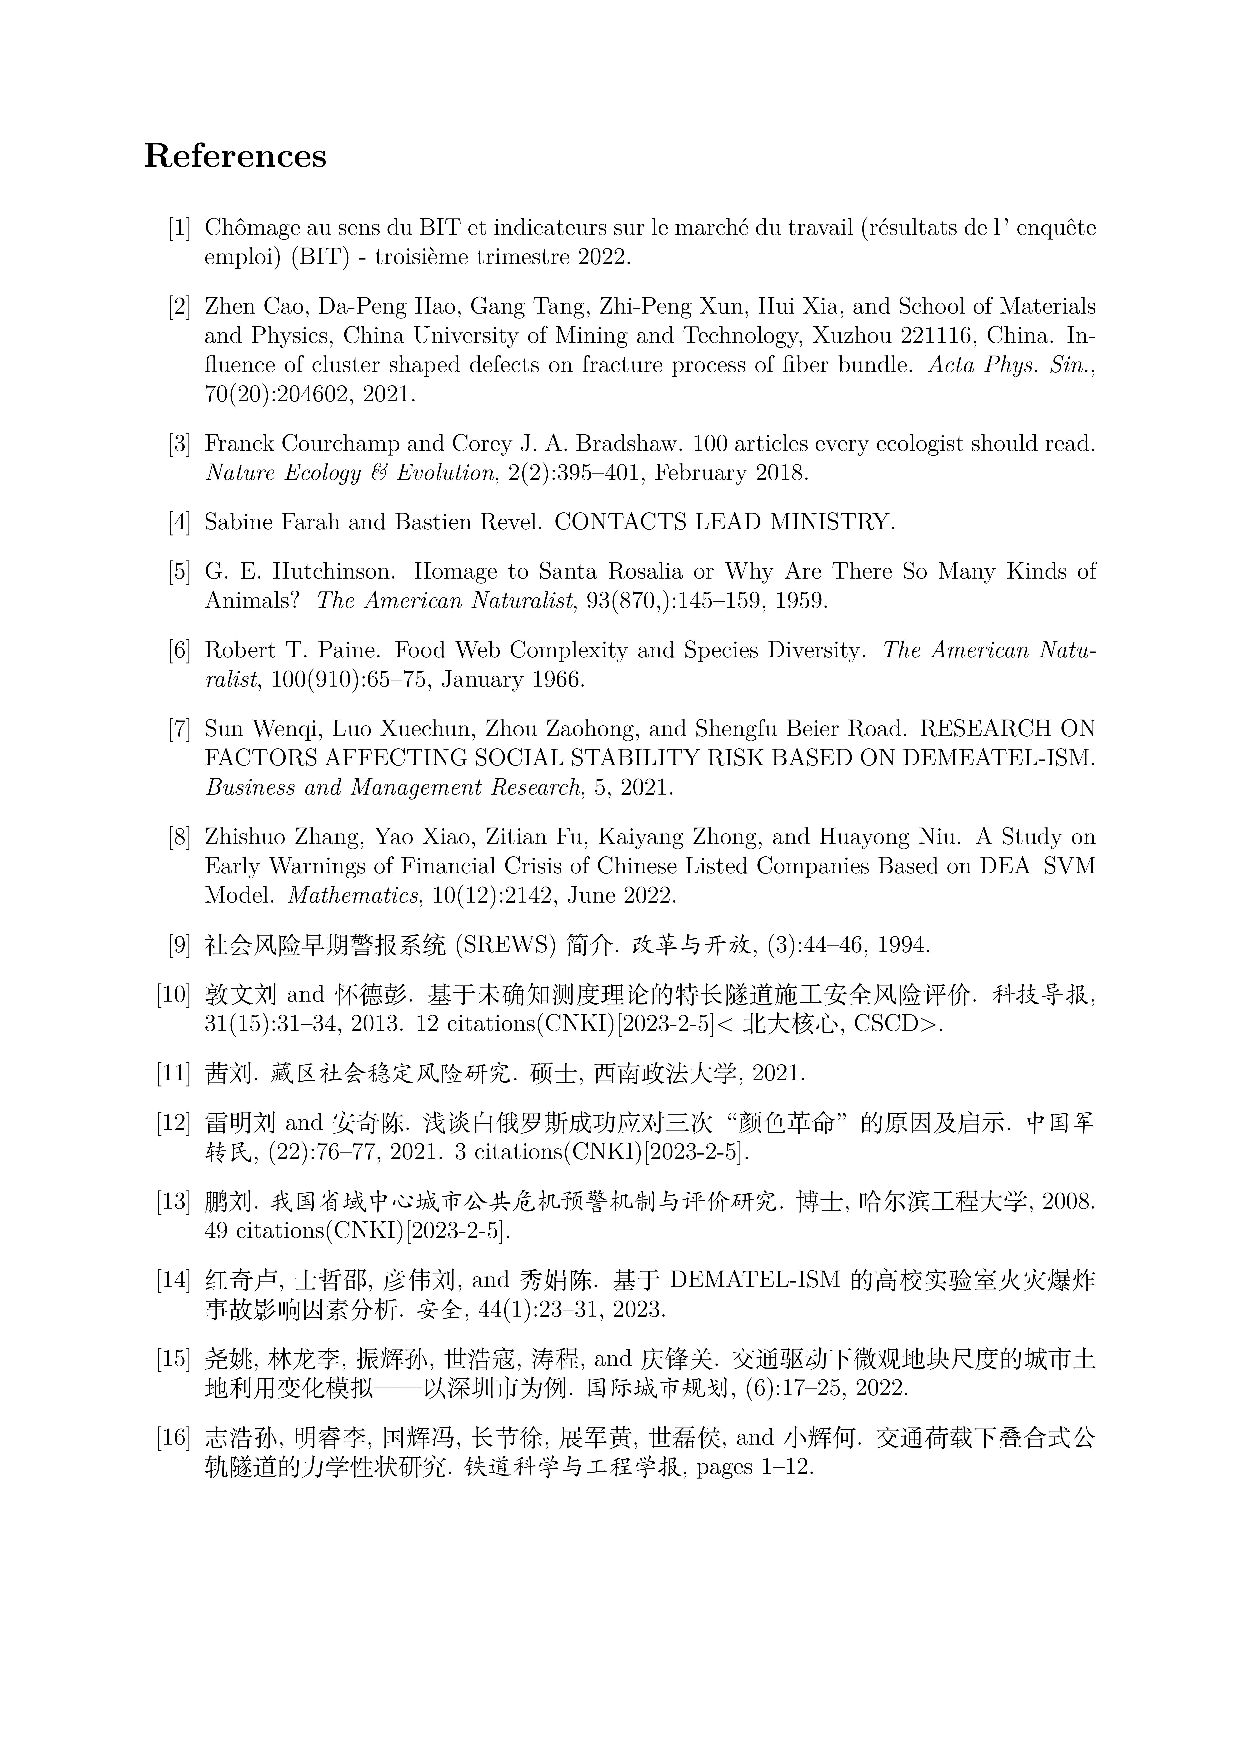
\includegraphics[width=15cm]{img/c1.pdf}  
% \end{figure}
% \newpage
% \begin{figure}[h!] 	
% \vspace{-0.8cm}   %调整图片与上文的垂直距离   
% \setlength{\belowdisplayskip}{10.pt} 	
% 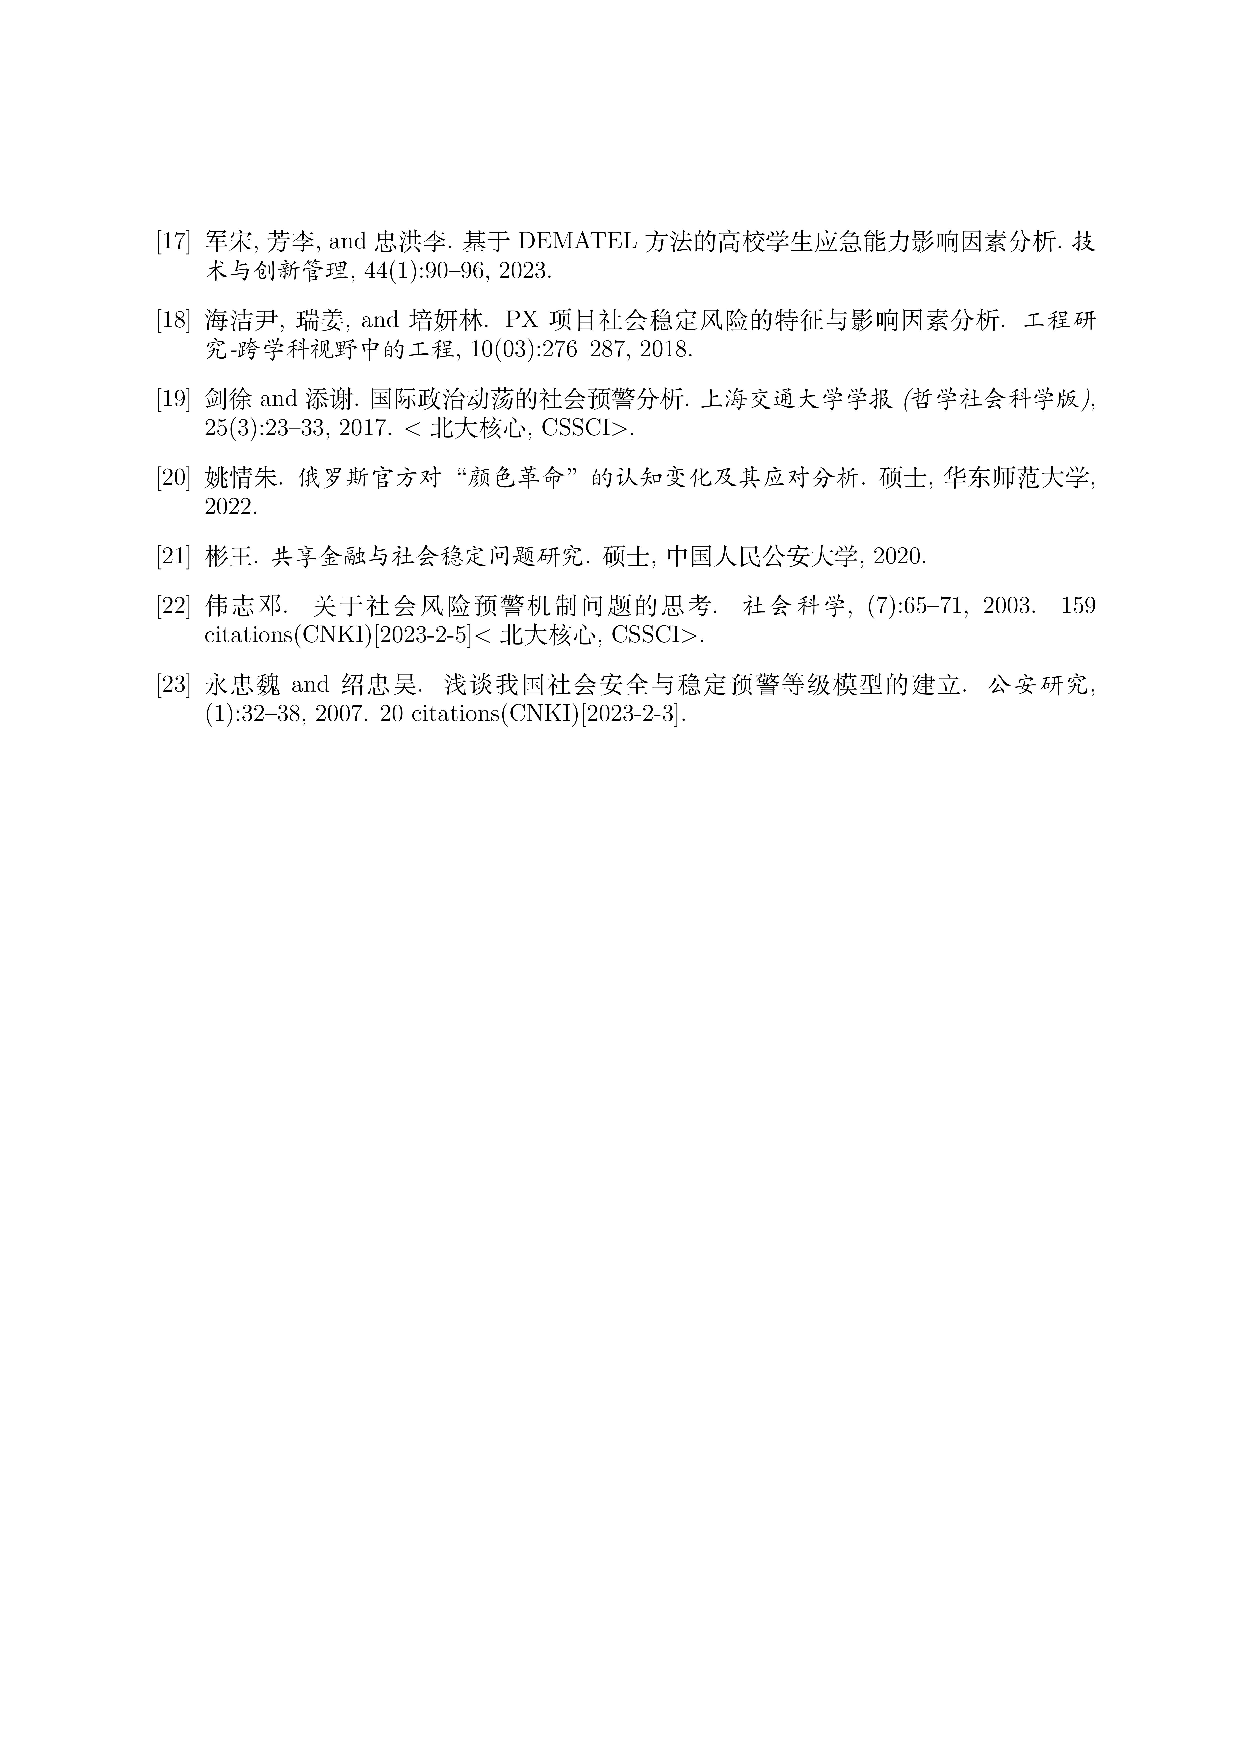
\includegraphics[width=15cm]{img/c2.pdf}  
% \end{figure}











\newpage
% 参考文献,此处以 MLA 引用格式为例
\begin{thebibliography}{100}

\bibitem{noauthor_chomage_nodate}
Chômage au sens du {BIT} et indicateurs sur le marché du travail (résultats
  de l’enquête emploi) ({BIT}) - troisième trimestre 2022.
\end{thebibliography}



% 以下为附录内容
% 如您的论文中不需要附录,请自行删除
\begin{subappendices}  % 附录环境
\section{Appendix}


\end{subappendices}  % 附录内容结束



















































\end{document}  % 结束
